\documentclass{beamer}

\input{../ts-glærur}

\title{FOR3R - Tímaflækjuskilgreiningar}

\begin{document}

\begin{frame}
\titlepage
\end{frame}

\section{Besta- versta og meðaltilfelli}

\begin{frame}{$\Theta$-notation: Óformleg skilgreining}
Í síðasta tíma lýstum við svokölluðu $\Theta$-notation til að lýsa vexti falla óformlega á eftirfarandi hátt:

\begin{center}
$\Theta(g(x))$ er mengi falla sem vaxa ``eins og $g(x)$.''
\end{center}

Þannig myndi t.d. $f(x) = 2 x^2 + 6$ vaxa eins og $x^2$, og þ.a.l. vera í menginu $\Theta(n^2)$. (Oft skrifað $f(x) = \Theta(n^2)$)
\end{frame}

\begin{frame}{Versti, besti og meðaltími}
\begin{itemize}
 \item Keyrslutími reiknirita fer oft ekki bara eftir stærð inntaks heldur líka eðli þess
 \begin{itemize}
  \item Besta tilfellið: Hversu hratt getur reikniritið mögulega keyrt?
  \item Versta tilfellið: Hversu lengi getur reikniritið mögulega keyrt? Oft áhugaverðasta tilfellið!
  \item ''Meðaltilfellið: Hversu langan tíma þarf reikniritið undir venjulegum kringumstæðum?
  \begin{itemize}
   \item Oft erfitt að skilgreina
   \item Oft ``random''
  \end{itemize}
 \end{itemize}
 \item Ath. að sama notation er notað í öllum tilfellum. Talað er um að reiknirit hafi gefinn keyrslutíma í ákveðnu tilfelli
 \item Dæmi: Reiknirit getur haft $\Theta(n)$ keyrslutíma í besta tilfellinu, en $\Theta(n^2)$ fyrir versta- og meðaltilfellið.
\end{itemize}
\end{frame}

\begin{frame}[fragile]{Dæmi um tímaflækju}
Skoðum eftirfarandi útfærslu á reikniritinu ``línuleg leit'':

\begin{minted}{python}
def linear_search(search_item, search_list):
    for i, item in enumerate(search_list):
        if item == search_item:
            return i
    return -1
\end{minted}

Það tekur inn lista með $n$ stökum og eitt stak sem á að leita að í listanum. Það skilar fyrsta vísi þar sem leitarstakið er jafnt staki í listanum, svo 
\begin{verbatim}
linear_search(x, l) 
\end{verbatim}
skilar tölunni $2$.

Hver er tímaflækja þessa reiknirits í besta, versta og meðaltilfellinu?

\end{frame}

\begin{frame}[fragile]{Dæmi um tímaflækju}
Skoðum eftirfarandi útfærslu á reikniritinu ``línuleg leit'':

\begin{minted}{python}
def linear_search(search_item, search_list):
    for i, item in enumerate(search_list):
        if item == search_item:
            return i
    return -1
\end{minted}

Það tekur inn lista með $n$ stökum og eitt stak sem á að leita að í listanum. Það skilar fyrsta vísi þar sem leitarstakið er jafnt staki í listanum, svo 
\begin{verbatim}
linear_search(4, [3, 2, 4, 1, 0, 4])
\end{verbatim}
skilar tölunni $2$.

Hver er tímaflækja þessa reiknirits í versta, besta og meðaltilfellinu á $\Theta$-formi?
\end{frame}

\begin{frame}[fragile]{Dæmi um tímaflækju}
Skoðum aðra útfærslu á línulegri leit. Þessi finnur alla vísana í listanum (ekki bara þann fyrsta):
\begin{minted}{python}
def linear_search_all(search_item, search_list):
    indices = []
    for i, item in enumerate(search_list):
        if item == search_item:
            indices.append(i)
    return indices
\end{minted}
Þannig að
\begin{verbatim}
linear_search_all(4, [3, 2, 4, 1, 0, 4])
\end{verbatim}
skilar listanum \texttt{[2, 5]}.

Hver er tímaflækja þessa reiknirits í versta, besta og meðaltilfellinu á $\Theta$-formi?
\end{frame}

\begin{frame}[fragile]{Python-ábending}
Hægt er að skrifa forritið á síðustu glæru á eftirfarandi hátt:
\begin{minted}{python}
def linear_search_all(search_item, search_list):
    for i, item in enumerate(search_list):
        if item == search_item:
            yield i
\end{minted}
Fallið skilgreinir þá svokallaðan \emph{generator}, sem skilar gildunum einu í einu. Þessi aðferð þykir betri þar sem henni er komið við, þar sem ekki þarf að búa til allan listann í minni.
\end{frame}


\section{Tímaflækjur: Formleg skilgreining}

\begin{frame}{$\Theta$-notation: Formleg skilgreining}
Skilgreinum $\Theta$-notation á eftirfarandi hátt:

Fyrir fall $g(n)$ er $\Theta(g(n))$ mengi af föllum. Til að fallið $f(n)$ sé í $\Theta(g(n))$ þurfa að vera til jákvæðir fastar $c_1$, $c_2$ og $n_0$ svo að $0 \leq c_1 g(n) \leq f(n) \leq c_2 g(n)$ fyrir öll $n \geq n_0$.

Á jöfnuformi:

\[\Theta(g(n)) = \{ f(n) : (\exists c_1, c_2, n_0 \in \mathbf{R}^+ :\]
\[0 \leq c_1 \cdot g(n) \leq f(n) \leq c_2 \cdot g(n), \forall n \geq n_0 )\}\]
\pause

\includegraphics[width=0.2\textwidth]{Pics/ewww}
\end{frame}

\begin{frame}{$\Theta$-notation: Mynd}
\begin{center}
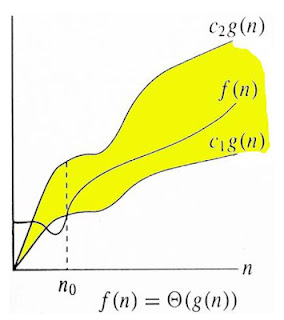
\includegraphics[width=0.5\linewidth]{Pics/ThetaAsympoticNotation}
\end{center}
$f(n) \in \Theta(g(n))$ ef hægt er að ``klemma'' $f(n)$ á milli $c_1g(n)$ og $c_2g(n)$ sé $n$ nógu stórt.

Hægt er að finna svona fasta með því að leysa ójöfnu.
\end{frame}

\begin{frame}{Markgildisskilgreining á $\Theta$-notation}
Önnur skilgreining á $\Theta$-notation er eftirfarandi:

\[
  f(n) \in \Theta(g(n)) \text{ ef } \lim_{n\to \infty}\frac{f(n)}{g(n)} = x, x \in \mathbf{R_+}
\]
Þetta getur verið auðveldara að reikna heldur en ójöfnur. $f(n) = \frac{1}{2}n^2 - 3n \in \Theta(n^2)$ af því að
\[
 \lim_{n\to \infty} \frac{\frac{1}{2}n^2 - 3n}{n^2} = \frac{1}{2}
\]
$\frac{1}{2} > 0$, svo $f(n) \in \Theta(n^2)$.
\end{frame}


\begin{frame}{$O$-notation: Skilgreining}
Þekktara en $\Theta$-notation er $O$-notation. Því svipar til $\Theta$-notation, en ólíkt $\Theta$-notation sem skorðar fall á milli tveggja falla þegar $n \to \infty$ gefur $O$-notation einungis efri mörk á vöxt fallsins.

Á jöfnuformi:

\[O(g(n)) = \{ f(n) : (\exists c_1, c_2, n_0 \in \mathbf{R}^+ : 0 \leq f(n) \leq c\cdot g(n), \forall n \geq n_0 )\}\]

eða

\[
  f(n) \in O(g(n)) \text{ ef } \lim_{n\to \infty}\frac{f(n)}{g(n)} < \infty
\]
\end{frame}


\begin{frame}{$O$-notation og önnur notation}
\begin{itemize}
 \item Ath. að þar sem $O$-notation setur ekki skorður á neðri mörk vaxtar fallsins er t.d. $n \in O(n^2)$
 \begin{itemize}
  \item $O$-notation er í ``daglegu tali'' oft notað eins og það sé $\Theta$-notation
 \end{itemize}
 \item Einnig er til...
 \begin{itemize}
  \item $\Omega$-notation, sem skorðar einungis neðri mörk fallsins
  \item $o$-notation og $\omega$-notation, sem gefa þrengri skorður
 \end{itemize}
\end{itemize}
\end{frame}

\begin{frame}{Önnur notkun}
\begin{itemize}
 \item Stundum er t.d. $O$- og $\Theta$-notation notað eins og þau séu föll frekar en mengi
 \item Sé reikniaðgerð ``notuð'' á t.d. $O(n)$ ber að skilja það sem ``fall í menginu $O(n)$
 \item Stundum notað til að tákna ''afgang`` 
 \item Dæmi: $2n^2 + 3n + 1$ má lýsa sem $2n^2 + \Theta(n)$
 \begin{itemize}
  \item Þetta gefur til kynna að liðirnir sem $\Theta(n)$ felur séu ekki markverðir.
 \end{itemize}
\end{itemize}
\end{frame}

\end{document}
